\ifx\wholebook\relax \else
% ------------------------

\documentclass[b5paper]{ctexart}
\usepackage[nomarginpar
  %, margin=.5in
]{geometry}

\addtolength{\oddsidemargin}{-0.05in}
\addtolength{\evensidemargin}{-0.05in}
\addtolength{\textwidth}{0.1in}

\usepackage[cn]{../../../prelude}

\setcounter{page}{1}

\begin{document}

\title{AVL树——证明和删除算法}

\author{刘新宇
\thanks{{\bfseries 刘新宇} \newline
  Email: liuxinyu95@gmail.com \newline}
  }

\maketitle
\fi

\markboth{AVL树——证明和删除算法}{基本算法}

\ifx\wholebook\relax
\chapter{AVL树——证明和删除算法}
\numberwithin{Exercise}{chapter}
\fi

\section{插入后的高度变化}

向AVL树插入元素后,高度变化存在四种情况:

\be
\begin{array}{rcl}
  \Delta H & = & |T'| - |T| \\
           & = & 1 + max(|r'|, |l'|) - (1 + max(|r|, |l|)) \\
           & = & max(|r'|, |l'|) - max(|r|, |l|) \\
           & = & \begin{cases}
\delta \geq 0, \delta' \geq 0: & \Delta r \\
\delta \leq 0, \delta' \geq 0: & \delta + \Delta r \\
\delta \geq 0, \delta' \leq 0: & \Delta l - \delta \\
\text{否则}: & \Delta l
\end{cases}
\end{array}
\ee

\begin{proof}
一次插入不可能同时增加左右分支的高度。平衡因子等于右子树的高度减去左子树的高度。根据其前后变化,共有四种情况:

\begin{enumerate}
\item 如果$\delta \geq 0$并且$\delta' \geq 0$,在插入前后,右子树的高度都不小于左子树的高度。高度的增加全部“贡献”自右子树的变化$\Delta r$;

\item 如果$\delta \leq 0$,在插入前左子树的高度不小于右子树,但是插入后$\delta' \geq 0$,说明右子树的高度由于插入增加了,而左子树保持不变($|l'|=|l|$)。所以高度的增加为:

\[
\begin{array}{rll}
\Delta H & = max(|r'|, |l'|) - max (|r|, |l|) & \{\delta \leq 0\ \text{且}\ \delta' \geq 0 \}\\
         & = |r'|-|l| & \{|l|=|l'|\}\\
         & = |r|+\Delta r - |l| & \\
         & = \delta + \Delta r & \\
\end{array}
\]

\item 如果$\delta \geq 0$且$\delta' \leq 0$,和情况二类似,我们有:

\[
\begin{array}{rll}
\Delta H & = max(|r'|, |l'|) - max (|r|, |l|) & \{\delta \geq 0\ \text{且}\ \delta' \leq 0 \}\\
         & = |l'|-|r| & \\
         & = |l| + \Delta l - |r| & \\
         & = \Delta l - \delta & \\
\end{array}
\]

\item 否则$\delta$和$\delta'$都不大于0,说明插入前后左子树的高度都不小于右子树。高度的增加全部“贡献”自左子树的变化$\Delta l$。
\end{enumerate}

\end{proof}

\section{插入后的平衡调整}

如图\ref{fig:avl-insert-fix-appendix}所示,所有需要修复的四种情况中,平衡因子都是$\pm 2$。调整后,平衡因子$\delta(y)$恢复为0。左右子树具有相同的高度。

\begin{figure}[htbp]
  \centering
  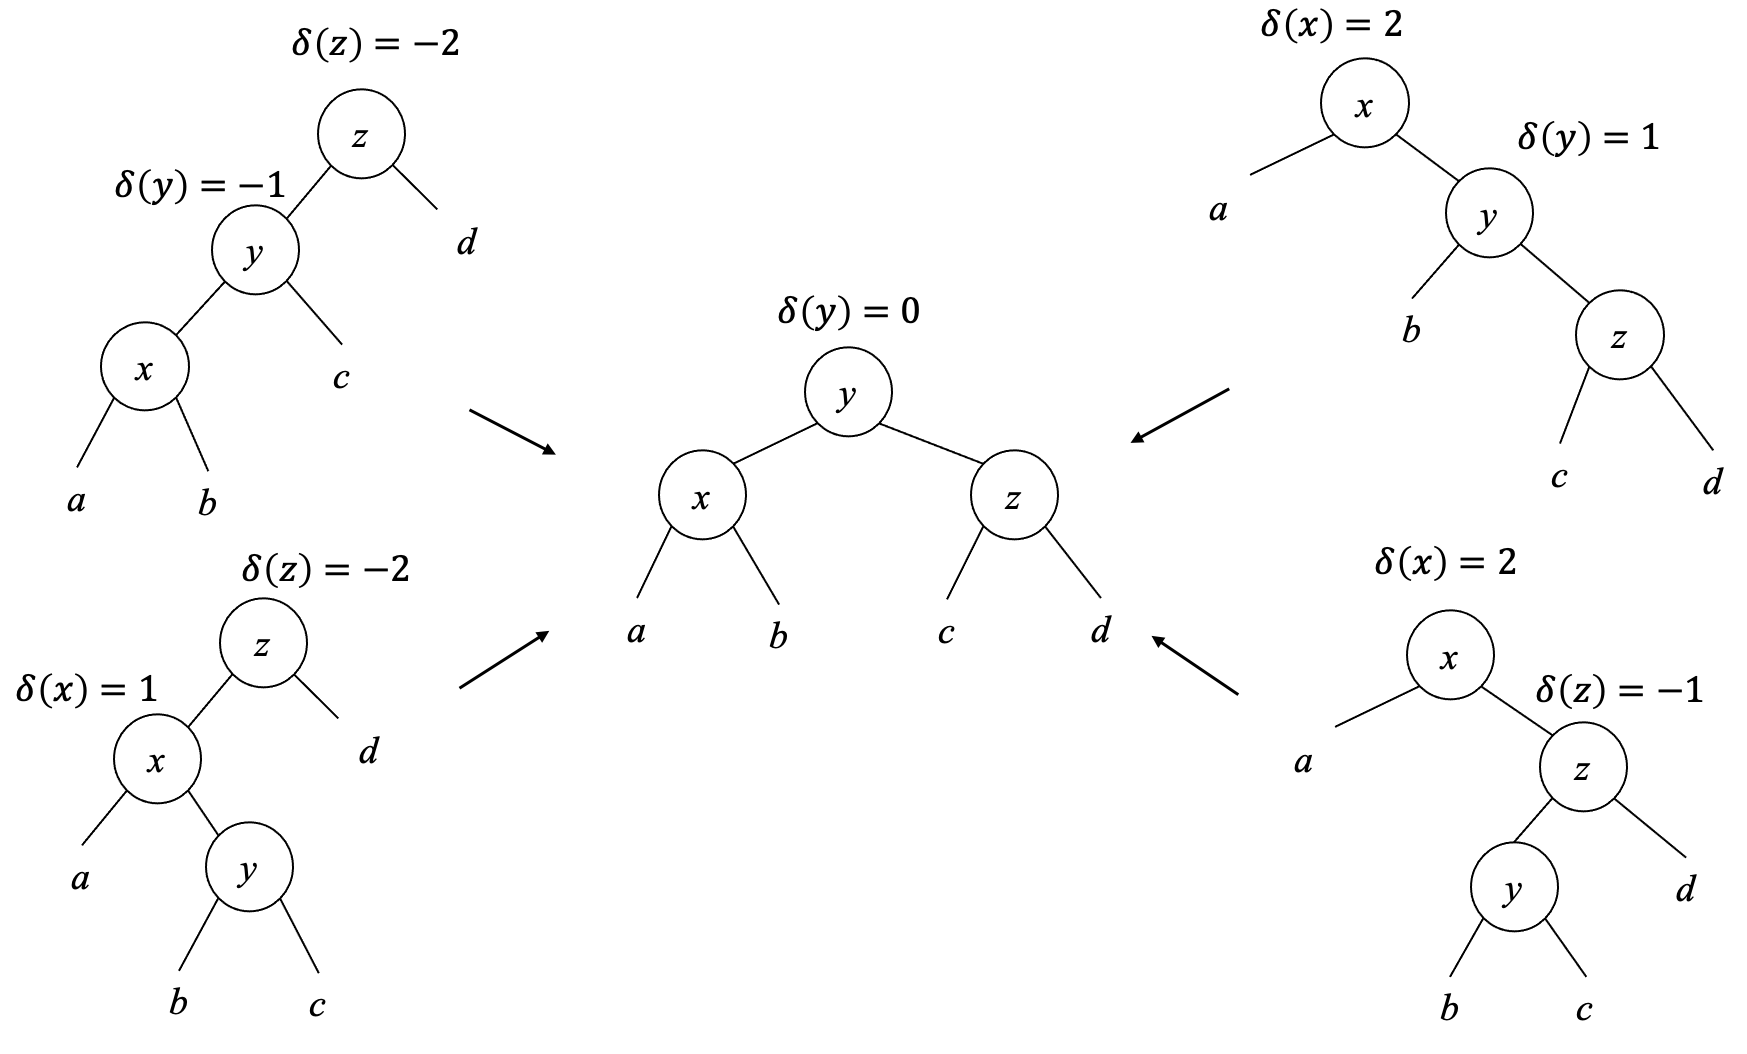
\includegraphics[scale=0.4]{../../../datastruct/tree/AVL-tree/img/avl-insert-fix.png}
  \caption{插入后需要恢复平衡的4种情况}
  \label{fig:avl-insert-fix-appendix}
\end{figure}

这4种情况分别是:左-左、右-右、右-左、左-右。记修复前的平衡因子分别为$\delta(x)$、$\delta(y)$、$\delta(z)$,修复后分别为$\delta'(x)$、$\delta'(y)$、$\delta'(z)$。我们接下来证明,调整后所有4种情况的平衡因子都变成$\delta(y)=0$。并且将给出$\delta'(x)$和$\delta'(z)$的结果。

\begin{proof}我们分别针对四种情况证明。

\textbf{左-左}

子树$x$在调整前后不变,因此$\delta'(x) = \delta(x)$。因为$\delta(y) = -1$且$\delta(z) = -2$,所以:

\be
  \begin{array}{rcl}
  \delta(y) = |c| - |x| = -1 & \Rightarrow & |c| = |x| - 1 \\
  \delta(z) = |d| - |y| = -2 & \Rightarrow & |d| = |y| - 2 \\
  \end{array}
  \label{eq:ll-cd}
\ee

调整后:

\be
  \begin{array}{rcll}
  \delta'(z) & = & |d| - |c| & \{ \text{式(\ref{eq:ll-cd})} \}\\
             & = & |y| - 2 - (|x| - 1) & \\
             & = & |y| - |x| - 1 & \{  x \text{是} y \text{的子节点} \Rightarrow |y|-|x| = 1\} \\
             & = & 0 & \\
  \end{array}
  \label{eq:ll-delta-z}
\ee

对于$\delta'(y)$,有如下结果:

\be
  \begin{array}{rcll}
  \delta'(y) & = & |z| - |x| & \\
             & = & 1 + max(|c|, |d|) - |x| & \{ \text{式(\ref{eq:ll-delta-z}), } |c| = |d|\} \\
             & = & 1 + |c| - |x| & \{ \text{式(\ref{eq:ll-cd})}\} \\
             & = & 1 + |x| - 1 - |x| & \\
             & = & 0 & \\
  \end{array}
\ee

汇总上述结果,对于左-左情况,新的平衡因子如下:

\be
  \begin{array}{l}
  \delta'(x) = \delta(x) \\
  \delta'(y) = 0 \\
  \delta'(z) = 0
  \end{array}
\ee

\textbf{右-右}

右-右和左-左对称,易知新的平衡因子结果如下:

\be
  \begin{array}{l}
  \delta'(x) = 0 \\
  \delta'(y) = 0 \\
  \delta'(z) = \delta(z)
  \end{array}
  \label{eq:rr-result}
\ee

\textbf{右-左}

首先考虑$\delta'(x)$。调整平衡后,我们有:

\be
  \delta'(x) = |b| - |a|
  \label{eq:rl-dx}
\ee

调整平衡前,$z$的高度为:

\be
  \begin{array}{rll}
  |z| & = 1 + max(|y|, |d|) &  \{ \delta(z) = -1 \Rightarrow |y| > |d|\} \\
      & = 1 + |y| & \\
      & = 2 + max(|b|, |c|)
  \end{array}
  \label{eq:rl-z}
\ee

因为$\delta(x) = 2$,所以:

\be
  \begin{array}{rll}
  \delta(x) = 2 & \Rightarrow |z| - |a| = 2 & \{ \text{式(\ref{eq:rl-z})} \}\\
                & \Rightarrow 2 + max(|b|, |c|) - |a| = 2 & \\
                & \Rightarrow max(|b|, |c|) - |a| = 0 &
  \end{array}
  \label{eq:rl-ca}
\ee

如果$\delta(y) = |c| - |b| = 1$,则:

\be
  max(|b|, |c|) = |c| = |b| + 1
\ee

将其代入式(\ref{eq:rl-ca})得到:

\be
  \begin{array}{ll}
  |b| + 1 - |a| = 0 \Rightarrow |b|-|a|= -1 & \{ \text{式(\ref{eq:rl-dx}) } \} \\
  \Rightarrow \delta'(x) = -1 &
  \end{array}
\ee

反之如果$\delta(y) \neq 1$,则$max(|b|, |c|) = |b|$,代入式(\ref{eq:rl-ca})得到:

\be
  \begin{array}{ll}
  |b| - |a| = 0  & \{ \text{式(\ref{eq:rl-dx})} \} \\
  \Rightarrow \delta'(x) = 0 &
  \end{array}
\ee

合并上述两种情况,我们得到$\delta'(x)$和$\delta(y)$的关系:

\be
\delta'(x) = \begin{cases}
  \delta(y) = 1: & -1 \\
  \text{否则}: & 0 \\
\end{cases} \\
\label{eq:rl-dx-dy}
\ee

对于$\delta'(z)$,根据定义它等于:

\be
  \begin{array}{rcll}
    \delta'(z) & = & |d| - |c| & \{ \delta(z) = -1 = |d| - |y| \} \\
               & = & |y| - |c| - 1 & \{ |y| = 1 + max(|b|, |c|) \} \\
               & = & max(|b|, |c|) - |c| \\
  \end{array}
  \label{eq:rl-dz}
\ee

如果$\delta(y) = |c| - |b| = -1$,则$max(|b|, |c|) = |b| = |c| + 1$。将其代入式(\ref{eq:rl-dz})中得到:$\delta'(z) = 1$。反之如果$\delta(y) \neq -1$,则$max(|b|, |c|) = |c|$,有$\delta'(z) = 0$。合并上述两种情况,$\delta'(z)$和$\delta(y)$的关系如下:

\be
  \delta'(z) = \begin{cases}
    \delta(y) = -1: & 1 \\
    \text{否则}: & 0 \\
    \end{cases} \\
  \label{eq:rl-dz-dy}
\ee

最后,对于$\delta'(y)$,我们可以推导出下面的关系:

\be
  \begin{array}{rl}
  \delta'(y) & = |z| - |x| \\
             & = max(|c|, |d|) - max(|a|, |b|)
  \end{array}
  \label{eq:rl-dy}
\ee

这里又分为三种情况:
\begin{enumerate}

\item 若$\delta(y)=0$,说明$|b|=|c|$,根据式(\ref{eq:rl-dx-dy})和式(\ref{eq:rl-dz-dy}),有:$\delta'(x)=0 \Rightarrow |a| = |b|$以及$\delta'(z)=0 \Rightarrow |c|=|d|$。因此$\delta'(y) = 0$。

\item 若$\delta(y)=1$,根据式(\ref{eq:rl-dz-dy}),我们有$\delta'(z)=0 \Rightarrow |c| = |d|$。

\[
  \begin{array}{rcll}
  \delta'(y) & = & max(|c|, |d|) - max(|a|, |b|) & \{|c|=|d|\} \\
             & = & |c| - max(|a|, |b|) & \{\text{式(\ref{eq:rl-dx-dy}): $\delta'(x)=-1 \Rightarrow |b|-|a|=-1$} \} \\
             & = & |c| - (|b| + 1) & \{ \delta(y) = 1 \Rightarrow |c|-|b|=1\} \\
             & = & 0 \\
  \end{array}
\]

\item 若$\delta(y)=-1$,根据式(\ref{eq:rl-dx-dy}),我们有$\delta'(x)=0 \Rightarrow |a|=|b|$。

\[
  \begin{array}{rcll}
  \delta'(y) & = & max(|c|, |d|) - max(|a|, |b|) & \{|a|=|b|\} \\
             & = & max(|c|, |d|) - |b| & \{ \text{式(\ref{eq:rl-dz-dy}): $|d|-|c|=1$} \} \\
             & = & |c| + 1 - |b| & \{  \delta(y) = -1 \Rightarrow |c|-|b|=-1\} \\
             & = & 0 \\
  \end{array}
\]

\end{enumerate}

全部三种情况的结果都是$\delta'(y)=0$。将上述结果归纳起来,可以得到新的平衡因子如下:

\be
  \begin{array}{l}
  \delta'(x) = \begin{cases}
    \delta(y) = 1: & -1 \\
    \text{否则}: & 0 \\
    \end{cases} \\
  \delta'(y) = 0 \\
  \delta'(z) = \begin{cases}
    \delta(y) = -1: & 1 \\
    \text{否则}: & 0 \\
    \end{cases} \\
  \end{array}
  \label{eq:rl-result}
\ee

\textbf{左-右}

左-右和右-左对称。使用类似的推导,我们可以得到和式(\ref{eq:rl-result})完全相同的结果。

\end{proof}

\section{删除算法}

删除后会引起子树高度的降低。如果平衡因子超出了$[-1, 1]$的范围,就需要修复以保持AVL树的性质。

\subsection{函数式删除}

我们先复用二叉搜索树删除算法,然后检查平衡因子并进行修复。删除的结果为一对值
$(T', \Delta H)$,其中$T'$是删除后的新树、$\Delta H$是高度的减少量。删除算法定义如下:

\be
delete = \textit{fst} \circ del
\ee

其中$del(T, k)$从树$T$种将元素$k$删除:

\be
\begin{array}{rcl}
del\ \nil\ k & = & (\nil, 0) \\
del\ (l, k', r, \delta) & = & \begin{cases}
  k < k': & tree\ (del\ l\ k)\ k'\ (r, 0)\ \delta \\
  k > k': & tree\ (l, 0)\ k'\ (del\ r\ k)\ \delta \\
  k = k': & \begin{cases}
    l = \nil: & (r, -1) \\
    r = \nil: & (l, -1) \\
    \text{否则}: & tree\ (l, 0)\ k''\ (del\ r\ k'')\ \delta \\
          & \text{其中}\ k'' = min(r) \\
  \end{cases} \\
\end{cases}
\end{array}
\label{eq:avl-del}
\ee

如果树为空,结果为$(\nil, 0)$;否则令树为$T = (l, k', r, \delta)$。我们比较$k$和$k'$的关系,并沿着子树递归查找和删除。当$k = k'$时,我们定位到了要删除的节点。如果它的任一子树为空,可以将其切下并用另一棵子树替代。否则,将右子树中的最小值$k''$切下,并替换$k'$。我们可以复用$tree$函数和$\Delta H$的结果。和插入算法相比,需要增加两种删除中特有的情况:

\begin{figure}[htbp]
  \centering
  \subcaptionbox{情况A}{
    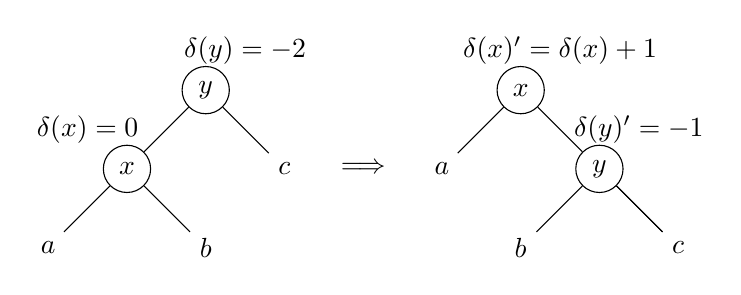
\begin{tikzpicture}[scale=1,
        trnode/.style={circle, draw, inner sep= 0pt, minimum size = .6cm}
      ]
      % left side
      \node[trnode] at (0, 0) (y) {$y$};
      \node[trnode] at (-1, -1) (x) {$x$};
      \draw (1, -1) node (c) {$c$};
      \draw (-2, -2) node (a) {$a$};
      \draw (0, -2) node (b) {$b$};
      % edges
      \draw (y) -- (x) -- (a);
      \draw (y) -- (c);
      \draw (x) -- (b);
      % labels
      \draw (0.5, 0.5) node{$\delta(y) = -2$};
      \draw (-1.5, -0.5) node{$\delta(x) = 0$};

      % right side
      \node[trnode] at (4, 0) (x1) {$x$};
      \draw (3, -1) node (a1) {$a$};
      \node[trnode] at (5, -1) (y1) {$y$};
      \draw (4, -2) node (b1) {$b$};
      \draw (6, -2) node (c1) {$c$};
      % edges
      \draw (x1) -- (y1) -- (c1);
      \draw (x1) -- (a1);
      \draw (y1) -- (b1);
      \draw (y1) -- (c1);
      % labels
      \draw (4.5, 0.5) node{$\delta(x)' = \delta(x) + 1$};
      \draw (5.5, -0.5) node{$\delta(y)' = -1$};

      \draw (2, -1) node{$\Longrightarrow$};
  \end{tikzpicture}} \\
  \subcaptionbox{情况B}{
    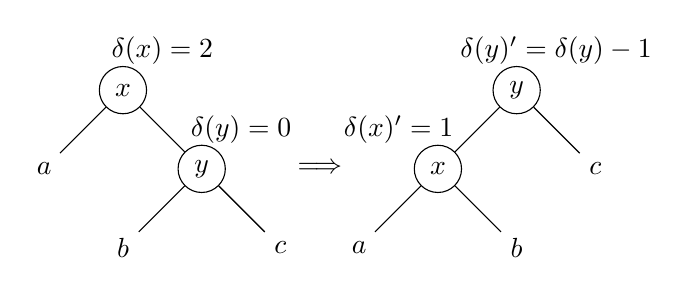
\begin{tikzpicture}[scale=1,
        trnode/.style={circle, draw, inner sep= 0pt, minimum size = .6cm}
      ]
      % left side
      \node[trnode] at (0, 0) (x) {$x$};
      \draw (-1, -1) node (a) {$a$};
      \node[trnode] at (1, -1) (y) {$y$};
      \draw (0, -2) node (b) {$b$};
      \draw (2, -2) node (c) {$c$};
      % edges
      \draw (x) -- (y) -- (c);
      \draw (x) -- (a);
      \draw (y) -- (b);
      \draw (y) -- (c);
      % labels
      \draw (0.5, 0.5) node{$\delta(x) = 2$};
      \draw (1.5, -0.5) node{$\delta(y) = 0$};

      % right side
      \node[trnode] at (5, 0) (y1) {$y$};
      \node[trnode] at (4, -1) (x1) {$x$};
      \draw (6, -1) node (c1) {$c$};
      \draw (3, -2) node (a1) {$a$};
      \draw (5, -2) node (b1) {$b$};
      % edges
      \draw (y1) -- (x1) -- (a1);
      \draw (y1) -- (c1);
      \draw (x1) -- (b1);
      % labels
      \draw (5.5, 0.5) node{$\delta(y)' = \delta(y) - 1$};
      \draw (3.5, -0.5) node{$\delta(x)' = 1$};


      \draw (2.5, -1) node{$\Longrightarrow$};
  \end{tikzpicture}}
  \caption{删除修复}
  \label{fig:avl-del-fixing}
\end{figure}

\be
\begin{array}{rcl}
 ... \\
balance\ ((a, x, b, \delta(x)), y, c, -2)\ \Delta H & = & (a, x, (b, y, c, -1), \delta(x) + 1, \Delta H) \\
balance\ (a, x, (b, y, c, \delta(y)),  2)\ \Delta H & = & ((a, x, b, 1), y, c, \delta(y) - 1, \Delta H) \\
  ... \\
\end{array}
\ee

相应的例子程序如下:

\lstset{frame = single}
\begin{Haskell}
delete t x = fst $ del t x where
  del Empty _ = (Empty, 0)
  del (Br l k r d) x
    | x < k = node (del l x) k (r, 0) d
    | x > k = node (l, 0) k (del r x) d
    | isEmpty l = (r, -1)
    | isEmpty r = (l, -1)
    | otherwise = node (l, 0) k' (del r k') d where k' = min r
\end{Haskell}

其中\texttt{min}和\texttt{isEmpty}定义为:

\begin{Haskell}
min (Br Empty x _ _) = x
min (Br l _ _ _) = min l

isEmpty Empty = True
isEmpty _ = False
\end{Haskell}

这样总共有7种情况需要在\texttt{balance}中实现:

\begin{Haskell}
balance (Br (Br (Br a x b dx) y c (-1)) z d (-2), dH) =
        (Br (Br a x b dx) y (Br c z d 0) 0, dH-1)
balance (Br a x (Br b y (Br c z d dz)    1)    2, dH) =
        (Br (Br a x b 0) y (Br c z d dz) 0, dH-1)
balance (Br (Br a x (Br b y c dy)    1) z d (-2), dH) =
        (Br (Br a x b dx') y (Br c z d dz') 0, dH-1) where
    dx' = if dy ==  1 then -1 else 0
    dz' = if dy == -1 then  1 else 0
balance (Br a x (Br (Br b y c dy) z d (-1))    2, dH) =
        (Br (Br a x b dx') y (Br c z d dz') 0, dH-1) where
    dx' = if dy ==  1 then -1 else 0
    dz' = if dy == -1 then  1 else 0
-- Delete specific
balance (Br (Br a x b dx) y c (-2), dH) =
        (Br a x (Br b y c (-1)) (dx+1), dH)
balance (Br a x (Br b y c dy)    2, dH) =
        (Br (Br a x b    1) y c (dy-1), dH)
balance (t, d) = (t, d)
\end{Haskell}

\subsection{命令式删除}

命令式删除使用树旋作来修复平衡。和插入相比,删除需要处理更多的情况。我们首先复用二叉搜索树删除,然后再修复子树高度变化引起的平衡问题。

\begin{algorithmic}[1]
\Function{Delete}{$T, x$}
  \If{$x = $ NIL}
    \State \Return $T$
  \EndIf
  \State $p \gets$ \Call{Parent}{$x$}
  \If{\Call{Left}{$x$} = NIL}
    \State $y \gets $ \Call{Right}{$x$}
    \State replace $x$ with $y$
  \ElsIf{\Call{Right}{$x$} = NIL}
    \State $y \gets $ \Call{Left}{$x$}
    \State replace $x$ with $y$
  \Else
    \State $z \gets$ \textproc{Min}(\Call{Right}{$x$})
    \State copy key and satellite date from $z$ to $x$
    \State $p \gets$ \Call{Parent}{$z$}
    \State $y \gets$ \Call{Right}{$z$}
    \State replace $z$ with $y$
  \EndIf
  \State \Return \Call{AVL-Delete-Fix}{$T, p, y$}
\EndFunction
\end{algorithmic}

删除节点$x$时,记$x$的父节点为$p$。如果任一子树为空,我们将$x$切下,取代为另一子树。否则,如果两棵子树都不为空,我们在右子树中找到最小值节点$z$,将其中的数据复制到$x$,然后将$z$切下。最后,我们调用\textproc{AVL-Delete-Fix},并传入根节点$T$、父节点$p$、和替换节点$y$。记父节点$p$的平衡因子为$\delta(p)$,删除后的平衡因子为$\delta(p)'$。它们之间的关系有三种不同的情况:

\begin{enumerate}
\item $|\delta(p)| = 0$、$|\delta(p)'| = 1$。虽然删除后子树的高度降低了,但是父节点仍然满足AVL树的性质。修复中止。

\item $|\delta(p)| = 1$、$|\delta(p)'| = 0$。删除前左右子树的高度差为1,删除后原来较高的树减小了1。左右子树现在高度相等。结果是父节点的高度也减小了1。我们需要继续自底向上更新树的高度。

\item $|\delta(p)| = 1$、$|\delta(p)'| = 2$。这说明删除后子树的高度差违反了AVL树的性质,我们需要通过树旋转来修复平衡。
\end{enumerate}

对于情况3,大部分修复和插入算法相同。我们需要针对图\ref{fig:avl-del-fixing}中所示的两种情况进行额外的处理。

\begin{algorithmic}[1]
\Function{AVL-Delete-Fix}{$T, p, x$}
  \While{$p \neq $ NIL}
    \State $l \gets$ \Call{Left}{$p$}, $r \gets$ \Call{Right}{$p$}
    \State $\delta \gets \delta(p)$, $\delta' \gets \delta$
    \If{$x = l$}
      \State $\delta' \gets \delta' + 1$
    \Else
      \State $\delta' \gets \delta' - 1$
    \EndIf
    \If{$p$ is leaf} \Comment{$l = r =$ NIL}
      \State $\delta' \gets 0$
    \EndIf
    \If{$|\delta| = 1 \land |\delta'| = 0$}
      \State $x \gets p$
      \State $p \gets$ \Call{Parent}{$x$}
    \ElsIf{$|\delta| = 0 \land |\delta'| = 1$}
      \State \Return $T$
    \ElsIf{$|\delta| = 1 \land |\delta'| = 2$}
      \If{$\delta' = 2$}
        \If{$\delta(r) = 1$} \Comment{右-右}
          \State $\delta(p) \gets 0$
          \State $\delta(r) \gets 0$
          \State $p \gets r$
          \State $T \gets $ \Call{Left-Rotate}{$T, p$}
        \ElsIf {$\delta(r) = -1$} \Comment{右-左}
          \State $\delta_y \gets \delta($ \Call{Left}{$r$} $)$
          \If{$\delta_y = 1$}
            \State $\delta(p) \gets -1$
          \Else
            \State $\delta(p) \gets 0$
          \EndIf
          \State $\delta($ \Call{Left}{$r$} $) \gets 0$
          \If{$\delta_y = -1$}
            \State $\delta(r) \gets 1$
          \Else
            \State $\delta(r) \gets 0$
          \EndIf
        \Else \Comment{删除特有,右-右}
          \State $\delta(p) \gets 1$
          \State $\delta(r) \gets \delta(r) - 1$
          \State $T \gets$ \Call{Left-Rotate}{$T, p$}
          \State break \Comment{高度不再变化}
        \EndIf
      \ElsIf{$\delta' = -2$}
        \If{$\delta(l) = -1$} \Comment{左-左}
          \State $\delta(p) \gets 0$
          \State $\delta(l) \gets 0$
          \State $p \gets l$
          \State $T \gets $ \Call{Right-Rotate}{$T, p$}
        \ElsIf {$\delta(l) = 1$} \Comment{左-右}
          \State $\delta_y \gets \delta($ \Call{Right}{$l$} $)$
          \If{$\delta_y = -1$}
            \State $\delta(p) \gets 1$
          \Else
            \State $\delta(p) \gets 0$
          \EndIf
          \State $\delta($ \Call{Right}{$l$} $) \gets 0$
          \If{$\delta_y = 1$}
            \State $\delta(l) \gets -1$
          \Else
            \State $\delta(l) \gets 0$
          \EndIf
        \Else \Comment{删除特有,左-左}
          \State $\delta(p) \gets -1$
          \State $\delta(l) \gets \delta(l) + 1$
          \State $T \gets$ \Call{Right-Rotate}{$T, p$}
          \State break \Comment{高度不再变化}
        \EndIf
      \EndIf
      \Comment{高度减小,继续自底向上更新}
      \State $x \gets p$
      \State $p \gets$ \Call{Parent}{$x$}
    \EndIf
  \EndWhile
  \If{$p = $ NIL} \Comment{删除根节点}
    \State \Return $x$
  \EndIf
  \State \Return $T$
\EndFunction
\end{algorithmic}

\begin{Exercise}
\Question{比较AVL树的命令式删除和插入,将共同的部分抽出,实现一个通用的AVL树修复算法。}
\end{Exercise}

\section{例子程序}

下面的例子程序实现了AVL树的删除算法:

\begin{lstlisting}[language = Bourbaki]
Node del(Node t, Node x) {
    if x == null then return t
    Node y
    var parent = x.parent
    if x.left == null {
        y = x.replaceWith(x.right)
    } else if x.right == null {
        y = x.replaceWith(x.left)
    } else {
        y = min(x.right)
        x.key = y.key
        parent = y.parent
        x = y
        y = y.replaceWith(y.right)
    }
    t = deleteFix(t, parent, y)
    release(x)
    return t
}
\end{lstlisting}

其中\texttt{replaceWith}的定义参见红黑树的部分。\texttt{release(x)}释放节点$x$的空间。修复函数的实现如下:

\begin{lstlisting}[language = Bourbaki]
Node deleteFix(Node t, Node parent, Node x) {
    int d1, d2, dy
    Node p, l, r
    while parent != null {
        d2 = d1 = parent.delta
        d2 = d2 + if x == parent.left then 1 else -1
        if isLeaf(parent) then d2 = 0
        parent.delta = d2
        p = parent
        l = parent.left
        r = parent.right
        if abs(d1) == 1 and abs(d2) == 0 {
            x = parent
            parent = x.parent
        } else if abs(d1) == 0 and abs(d2) == 1 {
            return t
        } else if abs(d1) == 1 and abs(d2) == 2 {
            if d2 == 2 {
                if r.delta == 1 {  // 右-右
                    p.delta = 0
                    r.delta = 0
                    parent = r
                    t = leftRotate(t, p)
                } else if r.delta == -1 { // 右-左
                    dy = r.left.delta
                    p.delta = if dy == 1 then -1 else 0
                    r.left.delta = 0
                    r.delta = if dy == -1 then 1 else 0
                    parent = r.left
                    t = rightRotate(t, r)
                    t = leftRotate(t, p)
                } else { // 删除特有,右-右
                    p.delta = 1
                    r.delta = r.delta - 1
                    t = leftRotate(t, p)
                    break // 高度不再继续变化
                }
            } else if d2 == -2 {
                if (l.delta == -1) { // 左-左
                    p.delta = 0
                    l.delta = 0
                    parent = l
                    t = rightRotate(t, p)
                } else if l.delta == 1 { // 左-右
                    dy = l.right.delta
                    l.delta = if dy == 1 then -1 else 0
                    l.right.delta = 0
                    p.delta = if dy == -1 then 1 else 0
                    parent = l.right;
                    t = leftRotate(t, l)
                    t = rightRotate(t, p)
                } else { // 删除特有,左-左
                    p.delta = -1
                    l.delta = l.delta + 1
                    t = rightRotate(t, p)
                    break // 高度不再继续变化
                }
            }
            // 高度减小,继续自底向上更新
            x = parent
            parent = x.parent
        }
    }
    if parent == null then return x // 删除根节点
    return t
}
\end{lstlisting}

\ifx\wholebook\relax \else
%% \begin{thebibliography}{99}

%% \bibitem{CLRS}
%% Thomas H. Cormen, Charles E. Leiserson, Ronald L. Rivest and Clifford Stein.
%% ``Introduction to Algorithms, Second Edition''. ISBN:0262032937. The MIT Press. 2001

%% \end{thebibliography}

\end{document}
\fi
